\chapter{Solution Design and Implementation}

This chapter describes the architecture that was designed for this project. In the first part of this chapter, a discussion on each of the individual parts that contribute to the stress test platform is presented. In the later stages of this chapter, an outline of some of the more relevant code snippets that make up the system is given and a discussion of how test-driven development helped in the development of this platform. The platform in question has been given the name "ws-flare". In this chapter when ws-flare is communicated, this is in reference to the platform that has been developed.

\section{Problem Definition}

This project aims to develop a tool for stress testing application which can easily integrate into continuous integration environments. The tool that we have created abstracts the complexities of stress testing, such as automatically scaling using Kubernetes, as well as automatic monitoring of applications in a microservice environment, ensuring that developers have better insights into how their applications handle an abundance of users. Throughout this chapter, the main technologies used to create this framework are presented.

\section{Technologies}

During the development of this platform, the following technologies have been utilized extensively.

\begin{itemize}
  \item NodeJS (Loopback 4)
  \item Angular
  \item Highcharts
  \item Docker
  \item Kubernetes
  \item MySQL
  \item RabbitMQ
  \item GraphQL
\end{itemize}

\subsection{NodeJS (Loopback 4)}

NodeJS was chosen for this project as it has a very low memory footprint when compared to languages such as Java. The reason this is important is that the platform has been developed using a microservice architecture, with many services contributing to the final product. The platform has also been exclusively developed to run on a kubernetes cluster. GKE (Google Kubernetes Engine) is a paid platform. In order to reduce financial costs while developing the platform, it is critical that the languages chosen have low memory consumption as that is the main cost factor involved when GKE calculates billing invoices.

The main NodeJS framework used in this project is Loopback 4 \cite{loopback4}. This is written in typescript and has inbuilt support for test-driven development.

\subsection{Angular}

Angular is a popular open source, single page application framework developed and maintained by Google \cite{angular}. This technoloogy is used for building the user interface of the ws-flare framework. Angular is written in typescript and comes with a powerful testing framework called TestBed which makes developing in a test-driven manner more straightforward.

\subsection{Highcharts}

In the ws-flare user interface, many graphs are displayed to show the results of test jobs. Highcharts is a charting library, developed by HighSoft \cite{highcharts}. It is free to use for open source applications and supports an abundance of graph visualizations.

\subsection{Docker}

Each service in the ws-flare framework is built to run in a docker container. This is necessary as the framework is built to run on a Kubernetes cluster which needs docker in order to function. Service are also deployed to Docker hub, which makes it easy for any company to import the framework into their environments as they are made publicly available.

\subsection{Kubernetes}

The ws-flare framework is built exclusively to run on Kubernetes clusters. This helps with scalability issues when simulating many thousands of connections as Kubernetes can run over many machines simultaneously. Kubernetes package manager, called Helm \cite{helm} is used for packaging the framework. With helm we can easily distribute the framework and companies can install it into their own infrastructure with ease.

\subsection{MySql}

MySql is used as the main persistence engine within the framework. Data includes web socket metadata such as successful, failed and dropped connections as well as data gathered during monitoring of cloud foundry services. MySQL is run in high availability mode. For this, there are two instances of MySql running at the same time. One instance is for reads and the other instance is for writes. The reason for this is there are a lot of writes occurring during test runs. For example, while simulating 30000 connections, it is necessary to persist data for each connection in a short timeframe. While this is happening, users need to use the user interface to view test runs in real time. When users view the interface they are mostly reading information from the database. High availability prevents any latency when viewing the user interface.

\subsection{RabbitMQ}

Ws-flare is built using a distributed microservices architecture. Some services within the framework need to be able to talk to each other. RabbitMQ is a messaging queue which makes this possible. Services are able to listen to topics in RabbitMQ and other services can send messages to the topics. Once a service detects that a message has been sent they can then react to that service. Message queues are often considered as fire and forget mechanisms for sending messages. A service sends a message and does not care what will react to that message. This ensures that services are highly decoupled.

\subsection{GraphQL}

GraphQL is a new technology developed by FaceBook. It is built as an alternative to REST and is suited to largely decoupled microservices. In the ws-flare user interface, it is necessary to query numerous amounts information to display results to a developer. With REST it would be necessary to send a request to each of the relevant services on the backend and aggregate the results on the user interface. With GraphQL however the user interface needs to send a query to one single service, and that service aggregate the data coming from the other services. This makes working with many microservices much simpler.

\section{Architecture}

There are a few terms going forward that need to be defined. Below is an explanation of these terms

\begin{itemize}
  \item \emph{Pod} Is a group of one or more docker containers with shared storage and network running within Kubernetes.
  \item \emph{JWT} stands for JSON Web Token is an open standard \href{https://tools.ietf.org/html/rfc7519}{RFC 7519} for securely transmitting data between 2 places in JSON format. For the purposes of this project, this is used for user authentication.
\end{itemize}

\begin{figure}[!h]
  \centering
    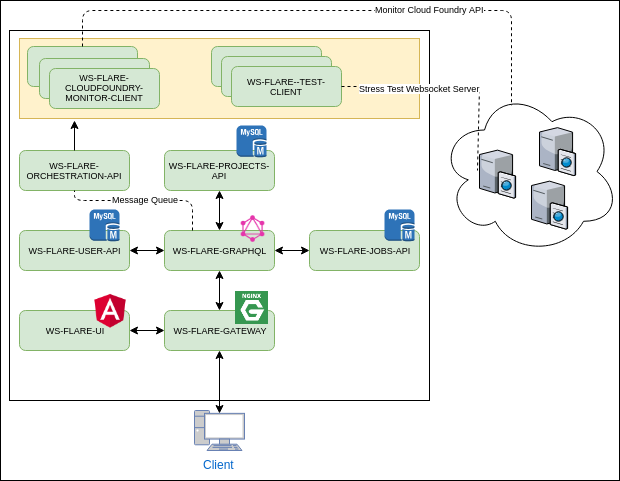
\includegraphics[width=0.8\textwidth]{figures/architecture.png}
    \caption{Architecture of the ws-flare platform}
    \label{fig:https-handshake}
\end{figure}

The project has been split up into a number of microservices to allow for maximum code readability and testability. The following microservices have been developed to make up the system.

\begin{itemize}
  \item ws-flare-ui
  \item ws-flare-user-api
  \item ws-flare-projects-api
  \item ws-flare-jobs-api
  \item ws-flare-orchestation-api
  \item ws-flare-cloud-foundry-monitor-api
  \item ws-flare-test-client
  \item ws-flare-cloudfoundry-monitor-client
  \item ws-flare-graphql
  \item ws-flare-gateway
  \item ws-flare-helm-chart
\end{itemize}

\subsection{ws-flare-ui}

This service is written in Angular. It holds all the code for displaying the user interface. Highcharts is also used as a charting library for displaying results.

\subsection{ws-flare-user-api}

This service holds all user authentication information, such as email, user-name, and passwords. For making authentication requests JWT tokens are utilized to allow a user to query the system. Without this security, the system would be exposed to hackers attempting to gain information.

\subsection{ws-flare-projects-api}

The system allows users to create projects to logically separate each task. This is more for user convenience and adds to the overall UX aesthetics's of the system. All project and task information are stored within this service. 

\subsection{ws-flare-jobs-api}

This service holds information about currently running jobs. The system allows for running multiple jobs at the same time to allow to be truly embedded into continuous integration environments.

\subsection{ws-flare-orchestation-api}

This service handles the orchestration of jobs. It is listening on a rabbitMQ message queue for requests to start new jobs. Once it has received a new request it calculates how many docker containers it needs to create in order to achieve the requested web socket load. It then instructs Kubernetes to start the required amount of pods that it needs to begin the stress test. It also instructs Kubernetes to start a pod designed specifically for monitoring Cloud Foundry applications. Once all pods have been created, finally the service instructs all pods to start the test and for the Cloud Foundry monitor to start monitoring the specified applications.

\subsection{ws-flare-cloud-foundry-monitor-api}

This service stores information related to running applications on Cloud Foundry, such as memory and CPU at a particular point in time. 

\subsection{ws-flare-test-client}

This service is dynamically created as a Kubernetes pod for the duration of a test run. The goal of this service is to simulate a number of web socket connections. A limit of 1000 connections per pod has been specified, this limitation was introduced to prevent the service from exceeding its assigned memory in Kubernetes. For example, if we have a test that requires a simulation of 5046 users then 6 ws-flare-test-client pods are created. Five of those simulate 1000 connections and the sixth simulates 46 connections. Together they simulate the full 5046 connections. For each of the connections established the connection information is stored within the ws-flare-jobs-api service. The service contains information on how many connections were successfully established, how many connections have dropped, and how many connections have not connected. Once the stress test has completed the service instructs Kubernetes to delete itself. Kubernetes then removes the pod.

\subsection{ws-flare-cloudfoundry-monitor-client}

This is another service that is created dynamically as a Kubernetes pod for the duration of a test run. Once it is created it immediately attempt to connect to the specified Cloud Foundry instance. There it attempts to find the applications that the user requested to monitor. Once the correct applications have been found the service sends a message to ws-flare-orchestation-api over a rabbitMQ message queue informing that it has found the correct applications and is ready to start monitoring. The application then waits for the orchestration API to create the necessary clients to simulate the Websockets. While the test is in progress the application actively communicates with the Cloud Foundry instance to interrogate it for applications statistics such as memory and CPU usage. It also gets information from each instance of the application deployed on cloud foundry. Once all tests have completed this service shuts itself down by instructing Kubernetes to kill itself. Kubernetes then removes the pod.

\subsection{ws-flare-graphql}

GraphQL was chosen in this architecture due to its ability to easily query multiple services at the same time in one request. Due to the need to present results to the user with minimal latency and very easy to integrate into Angular using apollo-client.

\subsection{ws-flare-gateway}

This is the API gateway to allow the user interface to communicate with the system. Using an API gateway provides a number of benefits, as everything is served through one endpoint or IP address. Currently, the gateway has routes only to the GraphQL server and the user interface server. The routes are outlined below

\begin{itemize}
  \item / routes to ws-flare-ui
  \item /graphql routes to ws-flare-graphql
\end{itemize}

The API gateway also provides a layer of security as the only way a user can interact with the system is through those 2 routes. It cannot communicate with any of the underlying services. The underlying technology of this gateway is an Nginx server \cite{nginx}.

\subsection{ws-flare-helm-chart}

This is the helm chart for the entire application. Helm is the package manager for Kubernetes. With helm we can define our entire infrastructure as code. This also provides anyone with a Kubernetes cluster to install the application with one single command as shown in listing \ref{code:helm-install}.

\begin{listing}[H]
    \caption{Install a helm chart with one single command using helm package manager}
    \label{code:helm-install}
    \begin{minted}{bash}
helm install .
\end{minted}
\end{listing}

Kubernetes automatically creates network routing between services using its internal DNS server. This makes Kubernetes a very attractive solution for distributing applications, and one of the main reasons Kubernetes was chosen for this project as well as its ability to scale services over a number of nodes.

\subsection{Utilizing Kubernetes API to test at scale}

Stress testing as the name suggests puts a lot of stress on resources. Not only is this true for the system that is being tested, it is also true for the system performing the test. To eliminate resource drain on the system that is performing the test we need to easily be able to scale the test out for maximum throughput. Using a NodeJS script as defined in listing \ref{code:single-machine-websocket-example} on a 16GB Memory Intel core I7 laptop the maximum web socket connections that could be achieved peaked at 10000 simultaneous web sockets. After this amount, it was observed that connections would either drop randomly or not connect at all to a web socket server. For this reason it is necessary to scale the test onto multiple machines in order to go beyond this limitation.

\begin{listing}[H]
    \caption{Websocket script run on a single machine}
    \label{code:single-machine-websocket-example}
    \begin{minted}{javascript}
var WebSocket = require('ws');

for (let i = 0; i < 100000; i++) {
    var ws = new WebSocket('ws://localhost:9002');

    ws.on('open', function open() {
        console.log('Opened socket ' + i);
        ws.send('PING');
    });

    ws.on('error', () => {
        console.log('Got error');
    });
}
\end{minted}
\end{listing}

To maximize the number of web sockets we can simulate we need a scalable system. This is made possible by Kubernetes. With Kubernetes we can easily create new pods to perform the simulations. Kubernetes has a powerful rest API which we can perform a POST request on, passing it the required information it needs to create a new pod. An example request is outlined in listing \ref{code:kubernetes-rest-api-create-pod-example}.

\begin{listing}[H]
    \caption{Request to create a new kubernetes pod}
    \label{code:kubernetes-rest-api-create-pod-example}
\begin{minted}{typescript}
kubernetesClient
  .api
  .v1
  .namespaces('default')
  .pod
  .post({
    body: {
      kind: "Pod",
      apiVersion: "v1",
      metadata: {
        labels: {
          app: 'ws-flare-test-client'
        },
        name: 'ws-flare-test-client-abc1'
      },
      spec: {
        containers: [
          {
            name: 'ws-flare-test-client-abc1',
            image: 'wsflare/ws-flare-test-client',
            env: [],
            resources: {
              requests: {
                cpu: '100m'
              }
            }
          },
        ]
      }
    }
  });
\end{minted}
\end{listing}

The script defined in listing \ref{code:kubernetes-rest-api-create-pod-example} requests that Kubernetes create a new Pod using the ws-flare-test-client docker container. We can also pass environment variables to this Pod. Using this API we can also specify how much CPU this pod is assigned. The expression of 100m means that this pod has one hundred millicpu. if 1000m is the equivalent of one CPU then we can say that this Pod is assigned one-tenth of the available CPU cycles. From testing the application this is a good amount of CPU cycles to simulate 1000 web sockets. 

Considering that making the request defined in listing \ref{code:kubernetes-rest-api-create-pod-example} to Kubernetes yields one Pod which can simulate 1000 web sockets, it now is possible that by increasing to 10 requests, the framework now has the opportunity to create 10000 simulated connections.

There are a number of options for obtaining a Kubernetes cluster. Kubernetes can be deployed on an AWS Compute cluster using Amazons web-tools. Pivotal also has its own flavor of Kubernetes in the form of Pivotal Container Service (PKS)\cite{pks}. However, in practice and while working on this project it was found that Google Kubernetes Engine (GKE) was one of the simpler Kubernetes clusters to set up. It should also be noted that all of the above are paid services, and can become expensive depending on how much resources are assigned to a cluster. 

To create a new cluster on GKE there are a few guidelines. The following assumes that a GKE account has already been created. The GKE dashboard can be found at \href{https://console.cloud.google.com}{https://console.cloud.google.com}

\begin{figure}[!h]
  \centering
    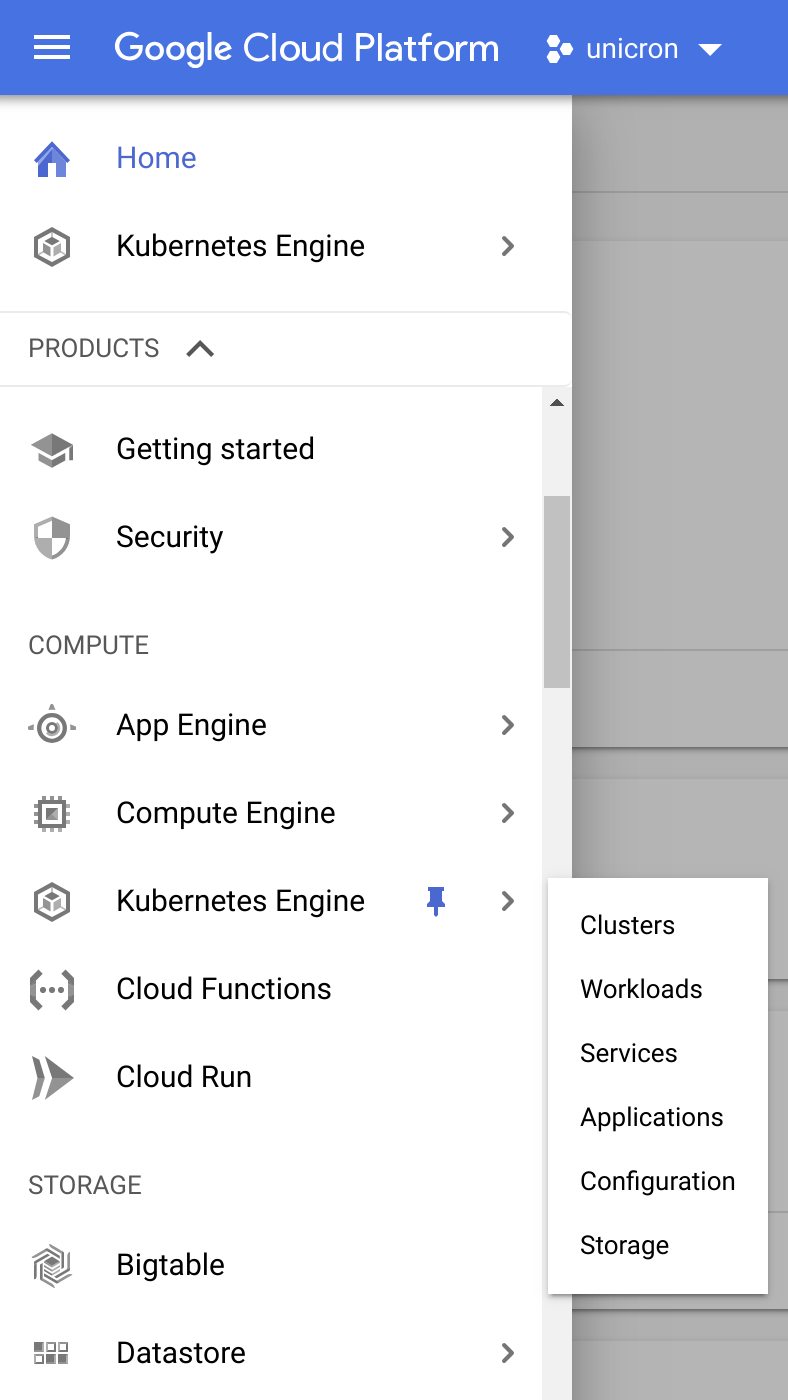
\includegraphics[width=0.5\textwidth]{figures/gke-setup-1.png}
    \caption{Select Kubernetes Engine then select Clusters}
    \label{fig:gke-setup-step-1}
\end{figure}

\FloatBarrier

Figure \ref{fig:gke-setup-step-1} brings a user to the Kubernetes engine screen where it is possible to create a new cluster

\begin{figure}[!h]
  \centering
    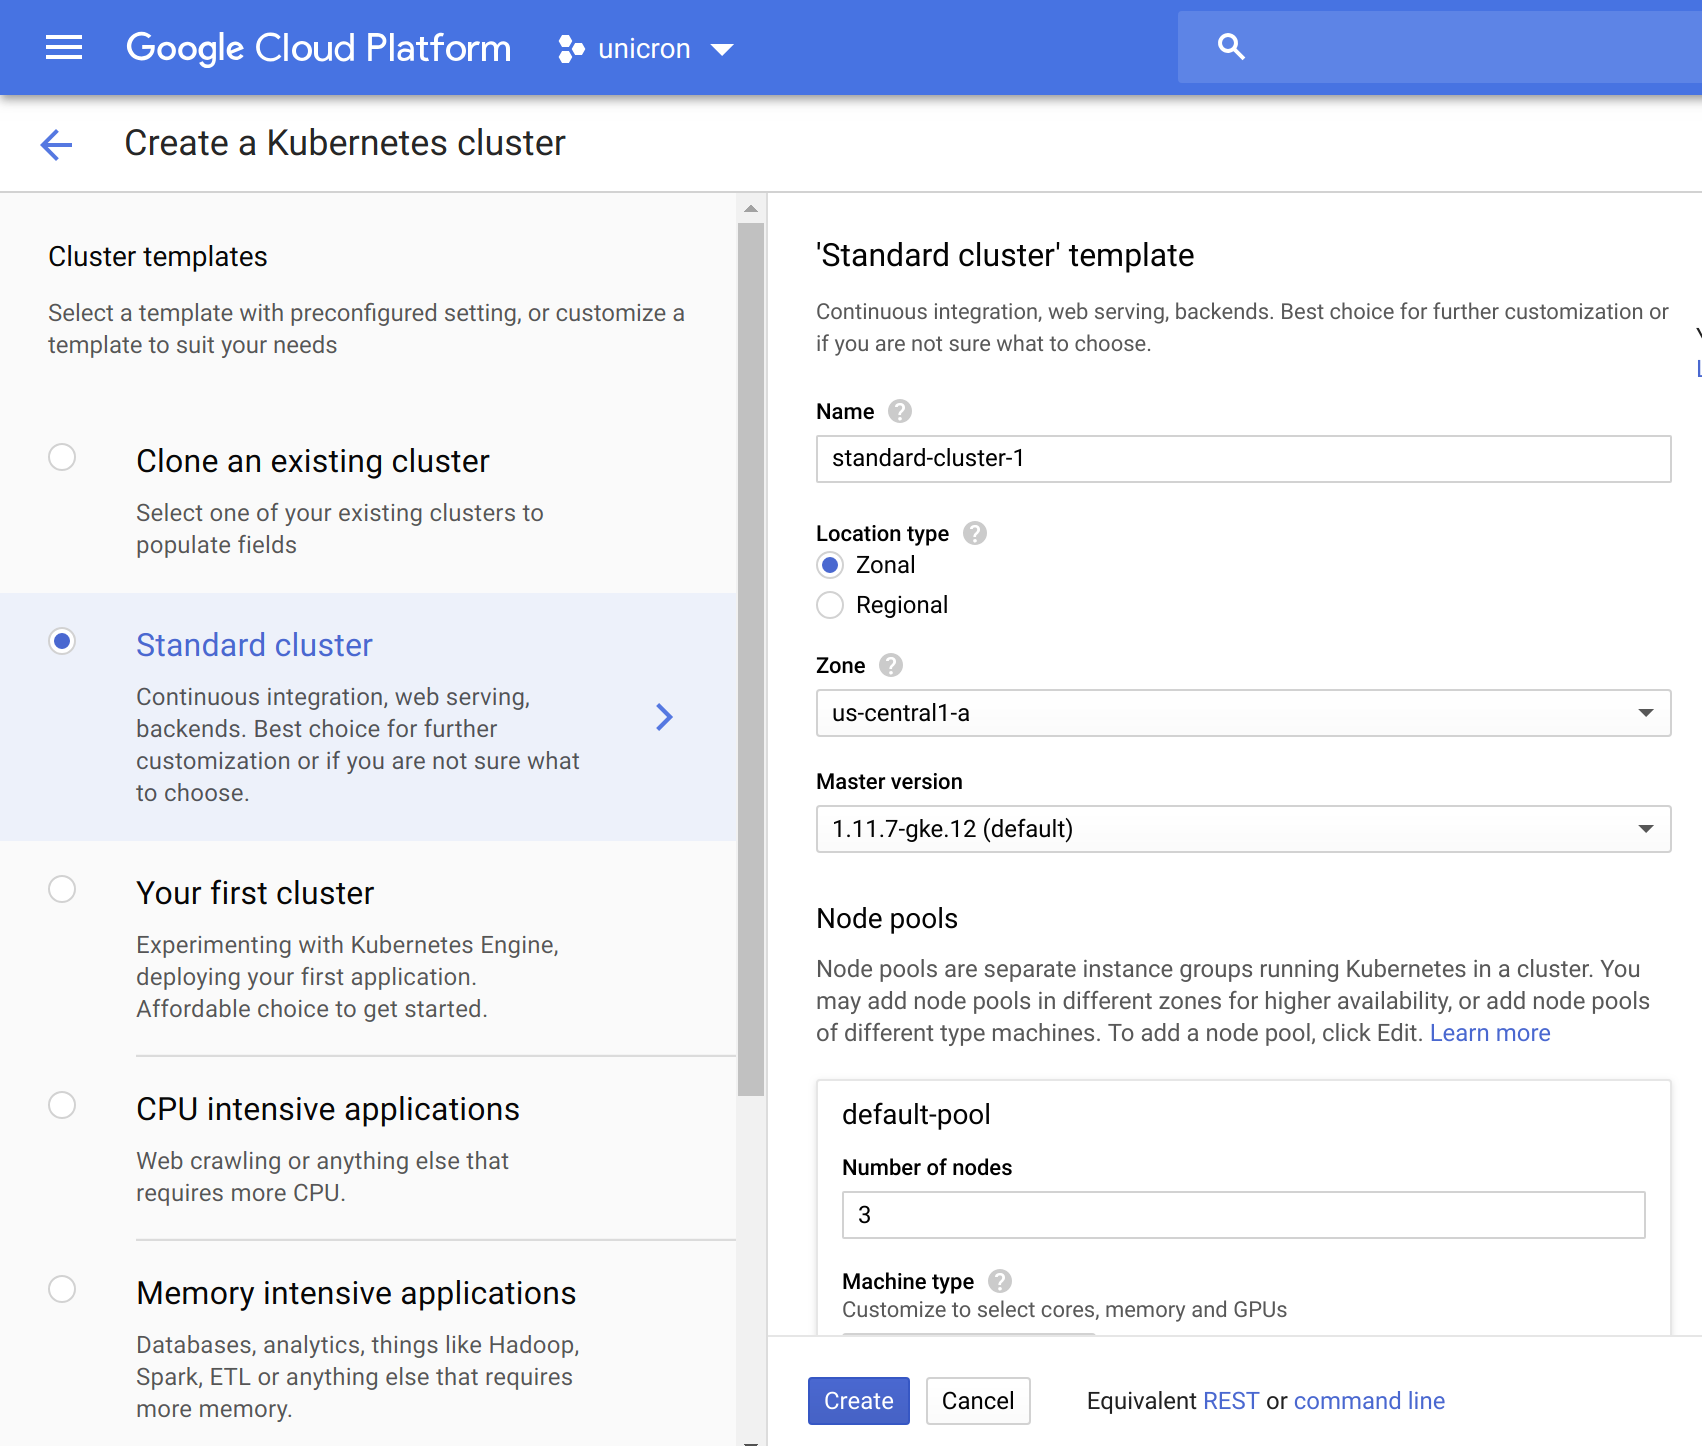
\includegraphics[width=0.8\textwidth]{figures/gke-setup-2.png}
    \caption{Select the resources to assign to this cluster}
    \label{fig:gke-setup-step-2}
\end{figure}

\FloatBarrier

Once the desired cluster resources and regional location of the cluster have been selected as depicted in figure \ref{fig:gke-setup-step-2}, click the Create button. After the cluster has been provisioned a user can connect to it. 

\begin{figure}[!h]
  \centering
    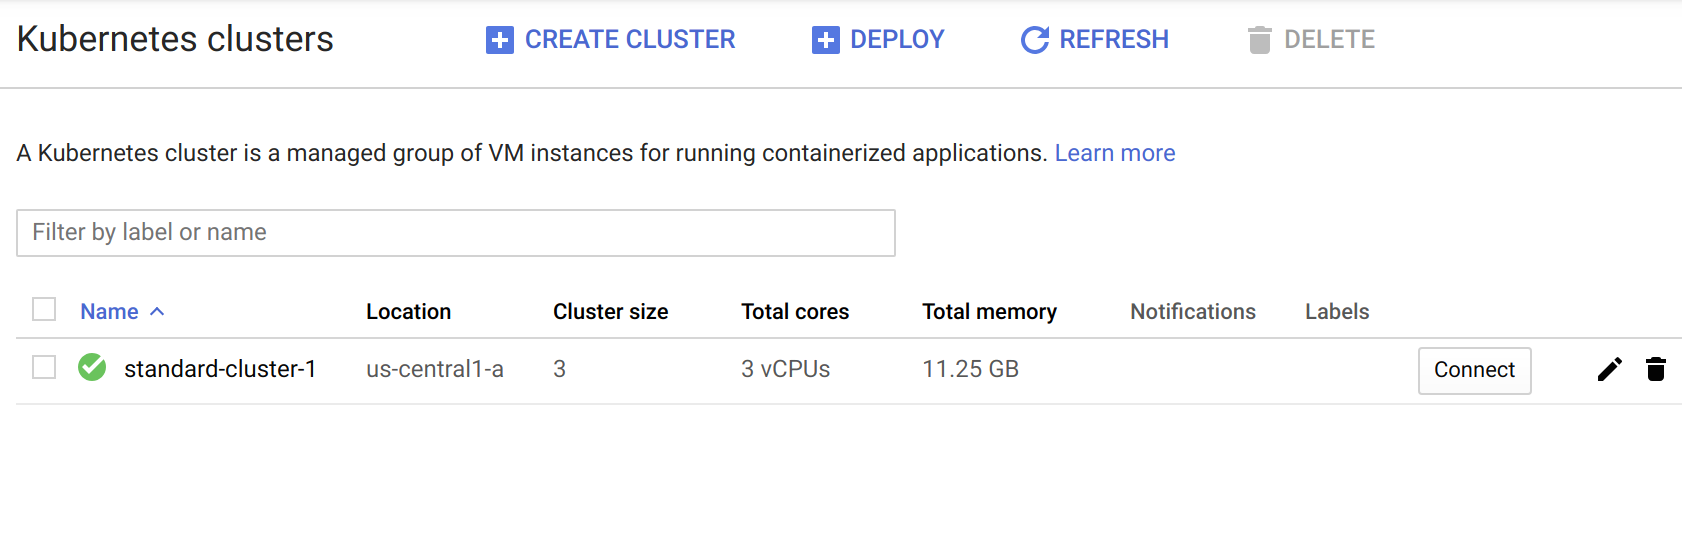
\includegraphics[width=0.8\textwidth]{figures/gke-setup-3.png}
    \caption{Click the connect button to get instructions on how to connect to the cluster}
    \label{fig:gke-setup-step-3}
\end{figure}

\FloatBarrier

After clicking connect as seen in figure \ref{fig:gke-setup-step-3}, a command is provided that can then be used to connect to the cluster from any comupter. Before running this command Google Cloud SDK tools needs to be installed. There is a quickstart guide available
\href{https://cloud.google.com/sdk/docs/quickstart-linux}{here}. Once the SDK tools are installed then the command that has been given from the GKE console should enable a successful connection to the cluster.

\subsection{Providing a scripting interface}

To ensure that it is possible to test a web socket server in a number of scenarios, the ws-flare platform allows users to script how they want the test to progress. This enables the user to simulate a number of scenarios. When users create a new task with the platform they are offered the opportunity to add a script. The script itself is a JSON array. An example of a valid script is shown in listing \ref{code:example-scripting-interface}.

\begin{listing}[H]
    \caption{An example of a script that can be used in the ws-flare testing framework}
    \label{code:example-scripting-interface}
    \begin{minted}{JSON}
[
    {
        "start": 0,
        "timeout": 55,
        "totalSimulators": 10000,
        "target": "wss://ws-flare-test-server.cfapps.io:4443"
    },
    {
        "start": 60,
        "timeout": 30,
        "totalSimulators": 5000,
        "target": "wss://ws-flare-test-server.cfapps.io:4443"
    },
    {
        "start": 120,
        "timeout": 60,
        "totalSimulators": 15000,
        "target": "wss://ws-flare-test-server.cfapps.io:4443"
    }
]
\end{minted}
\end{listing}

In this scenario, initially the system simulates 10000 connection to a web socket server. After 55 seconds, those 10000 connections disconnect and one minute into the test another 5000 connections attempt to connect to the server and disconnect after 30 seconds. Finally, 2 minutes into the test 15000 connection are simulated for one minute. Scripting is a very powerful feature of the stress testing platform. 

One scenario this feature can help to detect is the ability for a web socket server to actively clean up after itself when users disconnect. A potential scenario where this would have been applicable is having a web socket server backed by a Redis database. The role of the web socket server is to send notifications. Whenever a new web socket connected to the server the web socket server would create a new connection to the Redis database to wait for notifications. It was noticed that every hour the application would crash and restart automatically. After some investigation, it was found that the Redis connections were never dropped when a user disconnected their web socket. Over time the web socket server would simply be starved of memory and crash. With this scripting ability, we can actively test for this kind of scenario, among many other scenarios.

\subsection{Pivotal Cloud Foundry Monitoring}

As mentioned already, Cloud Foundry exposes a powerful API. As a ws-flare test is in progress the platform  actively attempts to gain valuable metrics from this API. The first thing that happens when the test begins is that the system attempts to log into cloud foundry using the user provided email and password. The login API endpoint request code is shown in listing \ref{code:example-pcf-login-script}

\begin{listing}[H]
    \caption{NodeJS script to login to Cloud Foundry}
    \label{code:example-pcf-login-script}
    \begin{minted}{typescript}
async login(authorization_endpoint: string): Promise<Token> {
    const token = await post('https://api.run.pivotal.io
/oauth/token', {
            headers: {
                Authorization: 'Basic Y2Y6',
                'Content-Type': 'application/x-www-form-urlencoded'
            },
            json: true,
            form: {
                grant_type: 'password',
                client_id: 'cf',
                username: this.cfUser,
                password: this.cfPass
            }
        });

    return token.content as any;
}
\end{minted}
\end{listing}

Using this code it is possible to get an access token that can be used to query the endpoints we need. A few important points, we need to set Basic Y2Y6 as an Authorization header and the correct Content-Type. It is also necessary to specify the grant\_type which in this case is password. Cloud Foundry offers a number of grant types such as password and Oauth. 

Cloud Foundry is split up into 3 logical entities. These are

\begin{itemize}
  \item Organizations
  \item Spaces
  \item Applications
\end{itemize}

Organizations represent a department in a company. The organization is the entity that is billed for the resources used on Cloud Foundry. On PWS (Pivotal Web Services) which is Pivotal's cloud offering of Cloud Foundry this is measured in both CPU usage and Memory usage over a period of a month.

Spaces represent different environments. Spaces make environment repeat-ability straightforward. For example there could be environments for DEV, STAGING and PROD  all with the same applications deployed and utilizing the same resources, however, they are used for very different functions. The DEV environment can be used by developers for testing code changes. The STAGING environment can be used by a quality assurance team to test any new features before reaching the PROD environment. the PROD environment is the last stop and this is the environment that the end user connects to.

Just like there can be multiple spaces in an organization, there can also be multiple applications deployed in space. The applications themselves are the applications that a developer writes. Applications on Cloud Foundry run in droplets, which are akin to Docker containers. Droplets require a user to specify a buildpack. Buildpacks are runtime environments for an application. Cloud Foundry supports many buildpacks for many different languages such as Java and NodeJS. To deploy an application to cloud foundry a user only needs to have an account and a manifest.yml file in the root of their project. A typical manifest file for a JAVA project looks like that defined in listing \ref{code:example-manifest-yaml}.

\begin{listing}[H]
    \caption{Example of a Cloud Foundry manifest file}
    \label{code:example-manifest-yaml}
    \begin{minted}{YAML}
name: test-application
instances: 1
memory: 1024M
path: build/libs/test-application-0.0.1-SNAPSHOT.jar
buildpack: java_buildpack
\end{minted}
\end{listing}

The name represents the name of the application on cloud foundry. The instances are the number of running instances of the application, this allows users to easily scale up their applications under heavy load. The memory field is the total amount of memory that this application is allowed to consume. If this limit is exceeded then an application will likely crash with an out of memory exception. The path is the path to the generated jar file for this Java project and the buildpack is the desired run time environment, which in this case is Java.

Once ws-flare has gained access to cloud foundry it is possible to use the given access token to interrogate applications running within a specified space. Each running application has a unique GUID assigned to it. To find these unique ids we first need to find which organization and space the applications are running in. We first retrieve the list of organizations using the code defined in listing \ref{code:example-cf-get-orgs}.

\begin{listing}[H]
    \caption{NodeJS script to retrieve a list of organizations from Cloud Foundry}
    \label{code:example-cf-get-orgs}
    \begin{minted}{typescript}
var response = json('https://api.run.pivotal.io/v2/organizations', {
    headers: {
        Authorization: token.token_type + ' ' + token.access_token,
        Accept: "application/json"
    }
});
\end{minted}
\end{listing}

The code defined in listing \ref{code:example-cf-get-orgs} yields a list of organizations running in Cloud Foundry that the user has access to. Each organization has a GUID which is a unique identifier. Once  the correct GUID is found its is possible to use this to search for the correct space by using the code defined in \ref{code:example-cf-get-spaces}

\begin{listing}[H]
    \caption{NodeJS script to retrieve a list of spaces from Cloud Foundry}
    \label{code:example-cf-get-spaces}
\begin{minted}[breaklines]{typescript}
var response = json('https://api.run.pivotal.io/v2/organizations/' + orgId + '/spaces', {
    headers: {
        Authorization: token.token_type + ' ' + token.access_token,
        Accept: "application/json"
    }
});
\end{minted}
\end{listing}

The code defined in listing \ref{code:example-cf-get-spaces} yields a list of spaces. Again each space has a unique GUID which can be used to get all the applications running within a space. To get a list of applications running within a space we can use code defined in listing \ref{code:example-cf-get-apps}

\begin{listing}[H]
    \caption{NodeJS script to retrieve a list of applications from Cloud Foundry}
    \label{code:example-cf-get-apps}
\begin{minted}[breaklines]{typescript}
var response =  json('https://api.run.pivotal.io/v2/spaces/' + spaceId +'/apps', {
    headers: {
        Authorization: token.token_type + ' ' + token.access_token
    }
});
\end{minted}
\end{listing}

Once the correct applications are found the last step is to use the obtained application GUID to get application statistics such as CPU and Memory usage. It is also possible to query the state of the application. There are 3 application states possible, these are, RUNNING, STOPPED and CRASHED. To get the information about a running application it is possible to use the script defined in listing \ref{code:example-cf-get-app-info}. 

\begin{listing}[H]
    \caption{NodeJS script to get information about an application running on Cloud Foundry}
    \label{code:example-cf-get-app-info}
\begin{minted}[breaklines]{typescript}
json('https://api.run.pivotal.io/v2/apps/' + appId + '/stats', {
    headers: {
        Authorization: token.token_type + ' ' token.access_token
    }
});
\end{minted}
\end{listing}

An example of a response from the script defined in listing \ref{code:example-cf-get-app-info} is outlined in listing \ref{code:example-cf-get-app-info-response}

\begin{listing}[H]
    \caption{Example response when interrogating application information on Cloud Foundry}
    \label{code:example-cf-get-app-info-response}
\begin{minted}[breaklines]{JSON}
{
  "0": {
    "state": "RUNNING",
    "isolation_segment": "iso-seg-name",
    "stats": {
      "usage": {
        "disk": 66392064,
        "mem": 29880320,
        "cpu": 0.13511219703079957,
        "time": "2014-06-19 22:37:58 +0000"
      },
      "name": "app_name",
      "uris": [
        "app_name.example.com"
      ],
      "host": "10.0.0.1",
      "port": 61035,
      "uptime": 65007,
      "mem_quota": 536870912,
      "disk_quota": 1073741824,
      "fds_quota": 16384
    }
  }
}
\end{minted}
\end{listing}

As can be seen in the response in listing \ref{code:example-cf-get-app-info-response}, there are some very useful metrics. The ws-flare-cloud-foundry-monitor-client continues to poll this endpoint for the duration of the stress test. Polling takes place every second. All results from a successful request are stored in a MySQL database for displaying the results over a period of time.

\section{Stress testing the web socket server}

For connecting to a live web socket server a popular NodeJS client called \href{https://www.npmjs.com/package/ws}{ws} is used. This is an intuitive client that has many useful features. For the purposes of this project, a number of metrics are monitored on a live web socket server.

\begin{itemize}
  \item Successful connection over a period of time
  \item Failed connections
  \item Dropped connections
\end{itemize}

NodeJS ws client offers some useful hooks when it comes to checking if a connection has successfully connected, failed or dropped as can be seen in listing \ref{code:example-ws-hooks}

\begin{listing}[H]
    \caption{Hooks provided by the ws library}
    \label{code:example-ws-hooks}
\begin{minted}[breaklines]{typescript}
const ws = new WebSocket('ws://www.host.com/path');
 
ws.on('open',  () => console.log('Successfully connected'));

ws.on('error',  () => console.log('Connection failed'));

ws.on('close' => console.log('Connection dropped'));
\end{minted}
\end{listing}

\subsection{Testing Frameworks Used}

Test Driven Development was used extensively throughout this project. The following tools were used for testing the various applications in the ws-flare system.

\begin{itemize}
  \item Yarn package manager for NodeJS 
  \item Mocha testing framework for NodeJS
  \item Docker for simulating MySQL and RabbitMQ
  \item CypressJS for end to end testing the user interface
  \item Jest for unit testing the user interface
  \item nyc for measuring typescript code coverage
\end{itemize}

For packaging each service into a docker container we made use of TravisCI \cite{travisCI} as a continuous integration pipeline. This tool is popular in the open source community and integrates well with GitHub which is the source code repository used for this project. When changes are made to any of the services Travis-ci automatically detects the changes and begins a build. Travis also detects if you have a .travis-ci.yaml configuration file on the root of your project. An example of a Travis configuration file is outlined in listing \ref{code:example-travis-yaml-file}.

\begin{listing}[H]
    \caption{Example travis configuration file}
    \label{code:example-travis-yaml-file}
\begin{minted}[breaklines]{yaml}
language: node_js
node_js:
  - '8'
services:
  - docker
install:
  - yarn --ignore-engines
  - docker pull mysql:5
script:
  - yarn test
  - docker build -t wsflare/ws-flare-projects-api:\$TRAVIS_BUILD_NUMBER .

after_success: yarn coverage

deploy:
  - provider: script
    script: docker login -u "\$DOCKER_USERNAME" -p "\$DOCKER_PASSWORD" && docker push wsflare/ws-flare-projects-api
    on:
      branch: master
\end{minted}
\end{listing}

The build goes through a number of steps. First, it installs all dependencies of the service using Yarn package manager. Next, it runs all tests, failing the build if any test fails. Next, docker build is run which packages the application into a docker container. Once this completes successfully Travis will release the docker container to docker hub which is a public registry for Docker containers. From there the docker container can be pulled into any project which is using docker or Kubernetes.

For monitoring code coverage this project uses a cloud offering called Coveralls \cite{coveralls}. This integrates with Travis-ci. Code overage metrics are gathered during builds and sent to coveralls for analysis. Coveralls then summarises the code coverage for the project and gives an overall code coverage metric ranging from 0 to 100\%. Coveralls is free to use with open source projects.